\chapter{Planificación}
En este capítulo detallaré todo lo relativo a la planificación y estimación del proyecto. 

\section{Metodología utilizada}
Desde que se empiezan a programar los primeros ordenadores en la historia, la programación siempre ha sido 
minguneada y considerada bastante lejos de una actividad científica. Todo empezó a cambiar cuando los scripts
permitían realizar cálculos como ninguna otra herramienta hasta el momento. Fue la matemática Margaret Hamilton 
quien planteó por primera vez que los sistemas informáticos tenían que integrar tres componentes: hardware, 
software y los usuarios que los iban a usar. Fue Margaret Hamiltonen, cuando se produce lo que conocemos como 
crisis del software en 1968 quien acuñó en la \textit{NATO Software Engineering Conference} el termino Ingeniería
al proceso de creación de software. En ese momento donde parecía que crear software duradero y escalable en el tiempo 
era misión imposible hizo que se invirtiera en investigación y se construyera conocimiento. Este conocimiento es lo que hoy 
llamamos Ingeniería de Software: herramientas, técnicas de especificación y diseño que nos permiten especificar, 
desarrollar, validar y evolucionar como en cualquier otra ingeniería.

Las metodologías ágiles presentan una forma distinta de trabajar y organizarse, adaptándose a las condiciones
cambiantes que puedan surgir, aprovechando estos cambios para obtener ventajas. Con este tipo de metodologías 
podemos dividir el trabajo en pequeñas piezas de manera que podemos ir realizándolos de forma incremental.

Se ha barajado utilizar una de las dos metodologías más empleadas en la industria: Scrum y eXtreme Programming. 
eXtreme programming ha sido descartada por la imposibilidad de aplicación en términos de tiempo y recursos humanos. 
Los roles y artefactos exigidos por esta metodología son indiscutiblemente para un equipo de desarrollo segmentado. 
Sin embargo y en comparación con Scrum es una metodología muy enfocada en el proceso de desarrollo. Obliga a 
desarrollar guiándose de pruebas, a programar en parejas y asegurar la calidad del código en todas las etapas.

Scrum en cambio se muestra más flexible. En el año 2001 que K. Schwaber y Mike Beedle publican el
primer libro sobre Scrum\cite{agile_book}: "Agile Software Development with Scrum" esta metodología se ha convertido en la
más utilizada para el desarrollo de software. Siendo precisos y prudentes tampoco es posible aplicar 
propiamente dicho Scrum en este proyecto... fundamentalmente por ser una persona a cargo de todo el proceso.

Por tanto, me he permitido crear mi propia metodología de desarrollo basándome en los tres valores fundamentales 
que ofrecen estas tecnologías:
\begin{itemize}
    \item \textbf{Transparencia}: en todo momento se ha de conocer en qué se está trabajando, que problemas se está teniendo y/o si 
    existe algún bloqueo asociado.
    \item \textbf{Inspección}: se ha de inspeccionar y no perder de vista el progreso para conseguir el objetivo. La 
    trazabilidad del trabajo nos la ofrece el SCV (source control versioning) en nuestro caso GitHub con incorporación
    de funcionalidad por pull request.
    \item \textbf{Adaptación}: poder reaccionar a tiempo a los cambios requeridos por los stakeholders.
\end{itemize}

Una buena forma de cumplir las características citadas anteriormente, es realizar el desarrollo guiado por pruebas, 
lo que se conoce por TDD, \textit{Test Driven Development}. Al emplear esta metodología garantizamos la calidad 
de lo programado, trasladamos los requisitos a las pruebas de forma que se convierten en la más fiable documentación.
Además tener una gran cobertura de código testeado nos permite poder refactorizar con asiduedad y garantizarnos 
no generar mucha deuda técnica.
Como se ha comentado en otro capítulo de esta memoria, este trabajo quiere prestarle especial atención al 
automatizaje de tareas y trabajos de infraestructura, la realización de un sistema que se integre continuamente 
(CI) hace que se proteja siempre el PMV ya que es requisito indispensable para seguir añadiendo funcionalidad 
que los test pasen lo que significa que se siguen manteniendo los requisitos anteriores al añadir nueva 
funcionalidad.

\section{Herramientas}
Para el contribuir con la segunda característica introspectiva citada anteriormente, necesitamos no perder
de vista el progreso para conseguir el objetivo. Se ha recurrido a utilizar un sistema de control de versiones,
sin discusión alguna GIT ha sido la herramienta seleccionada. Se hace necesario una forja donde respaldar nuestro 
código, GitHub ha sido la opción seleccionada para alojar el código y tener un registro de las issues y Pull Request. Estas
características también las pueden servicios como GitLab. Pero las características premium de GitHub que ofrece una cuenta
universitaria como los tableros Kanban, integración continua con GitHub Actions...

Haciendo uso de esta herramienta, se han definido unas serie de milestones que agrupan historias de usuario e issues o tareas a realizar. Los
incrementos en el trabajo se han ido realizando por medio de Pull Request y cada una de estas lleva enlazada una o varias
issues. Para tener una visión general del estado del proyecto se ha usado la herramienta Projects integrada en GitHub.

\subsection{Milestones}
Los milestones hacen referencia al conjunto de productos mínimamente viables que se van generando conforme se avanza en el
desarrollo del proyecto. Un milestone está formado por un conjunto de issues, se entiende finalizado un milestone cuando se
han contemplado todos los issues asociados.
Los milestones creados se pueden observar en el repositorio de GitHub y son los siguientes:
\begin{enumerate}
    \item \textbf{Infraestructura}: desarrollo de la integración continua que compila la memoria y comprobador ortográfico más
    historias de usuario iniciales.
    \item \textbf{Modelo de datos}: definición de las clases que conforman el dominio del problema, atendiendo al estado
    del arte. El PMV incluye también las redacciones pertinentes de los capítulos de la memoria y el pretexto a las decisiones
    técnicas elegidas para implementar la solución.
    \item \textbf{Interfaz de programación de aplicaciones}: es la estructura del modelo que representa la solución del problema
    y todas las operaciones posibles a realizar con ellas. Supondrá la capa de abstracción para acceder a los datos y que pueda
    ser utilizada por otros desarrolladores para construir aplicaciones con distintos objetivos.
    \item \textbf{Frontend}: creación de un sistema web que permita consumir el API satisfaciendo las necesidades de mis usuarios ficticios.
\end{enumerate}

\subsection{Historias de usuario}
Como estamos trabajando con una metodología de desarrollo ágil queremos expresar las necesidades reales del sistema para lograr la interacción del equipo de desarrollo con el usuario. Ello se consigue por medio de historias de usuario, en adelante HU. Las HUs tienen que cumplir una serie de condiciones \cite{dddjj}:
\begin{itemize}
    \item Se tiene que identificar para que usuario se va a desarrollar la historia.
    \item La HU siempre está en el dominio del problema y siempre es narrada desde el punto de vista de ese usuario. Tiene que expresar el beneficio que obtendrá dicho usuario cuando se haya implementado la HU.
    \item La HU mayormente requiere la programación de cierta lógica de negocio. 
\end{itemize}
Todo lo que no cumpla estas características no son más que tareas enmarcadas en el proceso de desarrollo.

En este trabajo, todas las historias de usuarios están definidas en un milestone
de trabajo y de ellas se generarán tareas específicas. La especificación de las historias de usuario e issues generadas a partir de ellas
pueden verse con mayor detalle en el panel de \textbf{Issues} del repositorio de GitHub.
\begin{figure}[]
	\centering
	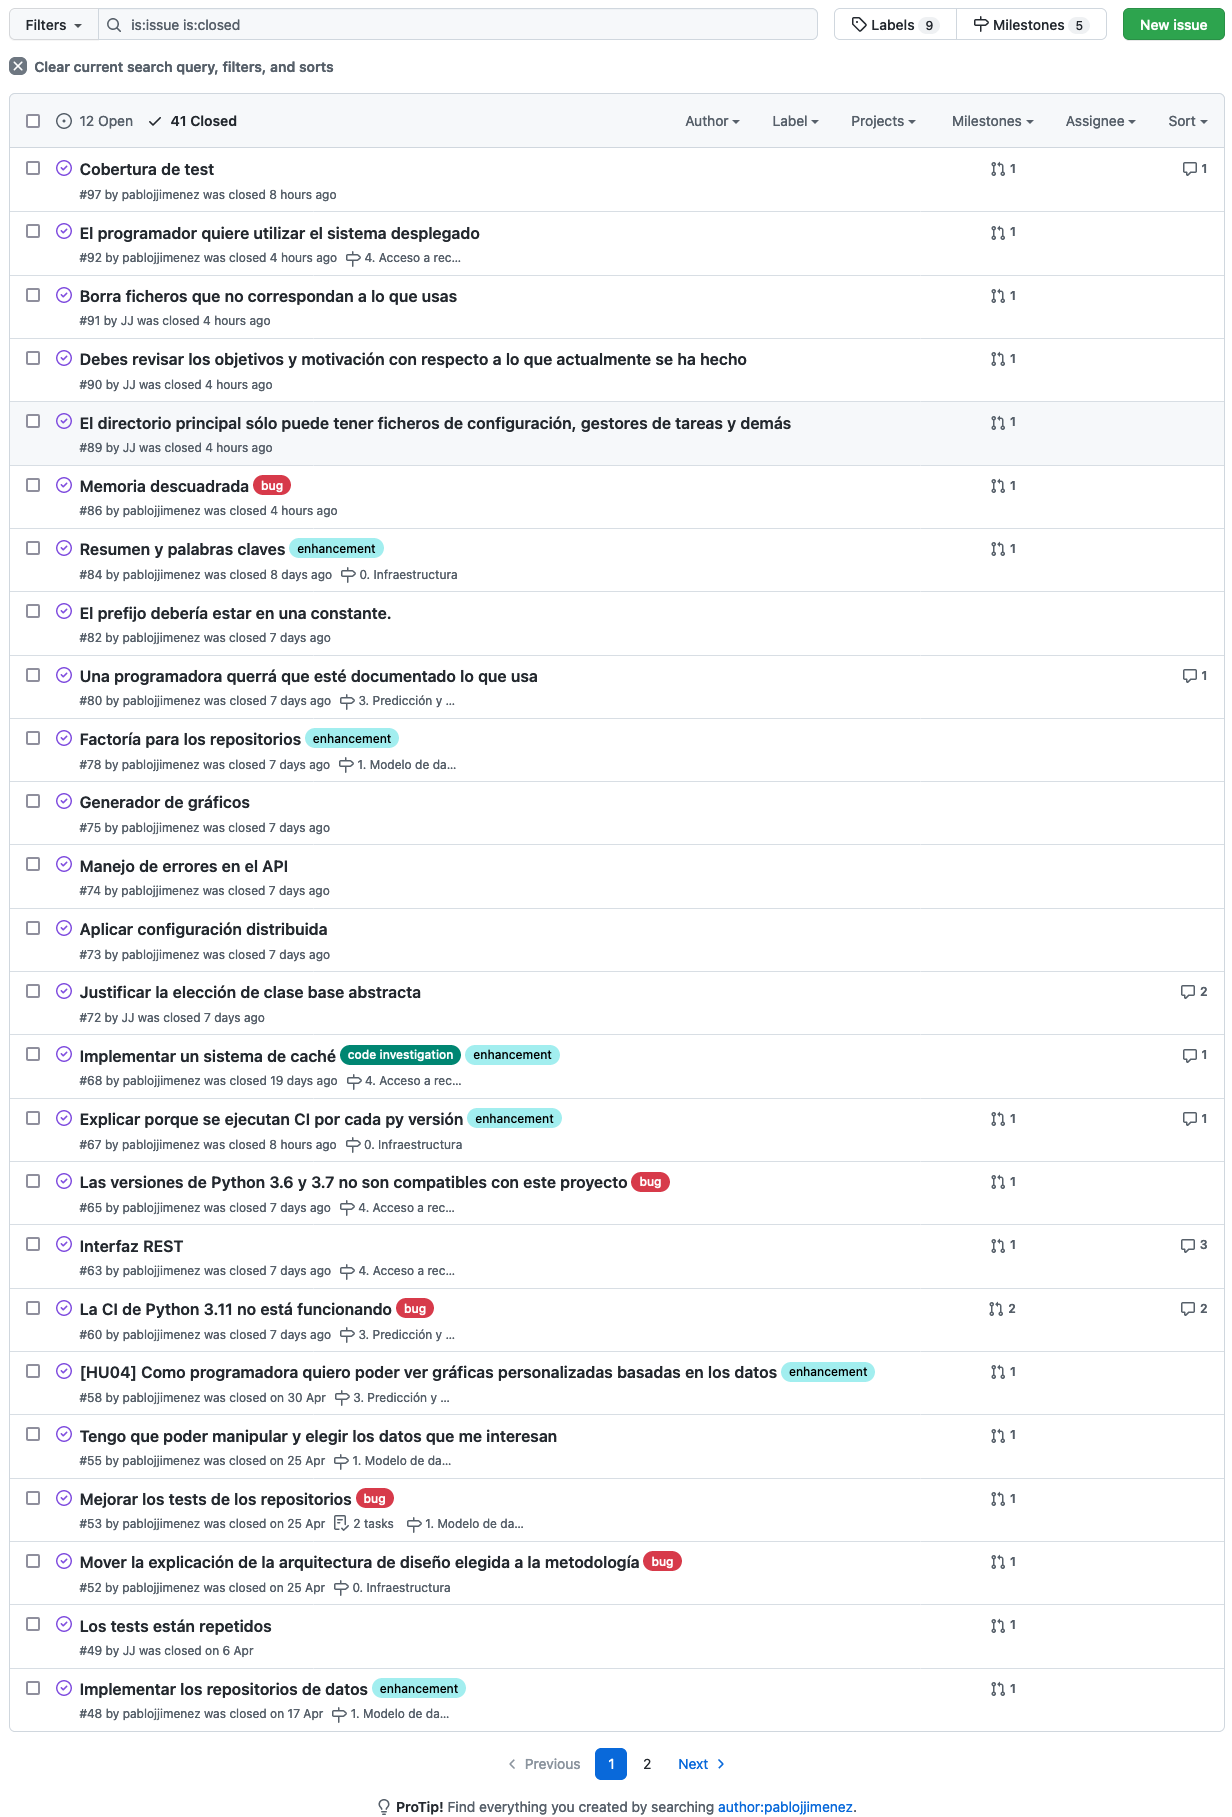
\includegraphics[scale=0.3]{doc/logos/imgs/issues.png}
	\caption{ Issues del TFG vistas desde el correspondiente \href{https://github.com/pablojjimenez/TFG/issues}{panel en GitHub}. }
    \label{fig:worst_f_value}
\end{figure}

\subsection{Cuantización de las horas empleadas}
[TODO: añadir algún gráfico procedente del CSV que vamos realizando]

\section{Estimación de costes}
A partir de la información anterior en cuanto al tiempo invertido en el proyecto y en vista de los elementos necesarios
para llevarlo a cabo podemos detallar los costes asociados que tendría la elaboración del proyecto.

\begin{itemize}
    \item MacBook Pro [amortizado 5 años]: 240€
    \item Recursos software utilizados han sido gratuitos.
    \item Despliegue: 25\$/mes. Se puede consultar el detalle en \hyperref[sec:despliegue]{el capítulo 5, sección sobre el coste.}
\end{itemize}
